\documentclass[conference]{IEEEtran}
\IEEEoverridecommandlockouts
% The preceding line is only needed to identify funding in the first footnote. If that is unneeded, please comment it out.
\usepackage{cite}
\usepackage[portuges,brazil,english]{babel}
\usepackage{amsmath,amssymb,amsfonts}
\usepackage{algorithmic}
\usepackage{graphicx}
\usepackage{textcomp}
\usepackage{float}
\def\BibTeX{{\rm B\kern-.05em{\sc i\kern-.025em b}\kern-.08em
    T\kern-.1667em\lower.7ex\hbox{E}\kern-.125emX}}
\begin{document}

\title{Linear Regression by Gradient Descent}

\author{\IEEEauthorblockN{Carolina Cuba}
\IEEEauthorblockA{
???? \\
????@????}
\and
\IEEEauthorblockN{Leonardo de Melo João}
\IEEEauthorblockA{
228118 \\
l228118@g.unicamp.br}}

\maketitle

\section{Methodology}

\subsection{Data Preparation}	
    A requirement for any computerized regression technique is that all data needs to be placed in discretized values and, in our case, three columns were presented as classes: cut, color and clarity. Fortunately, the semantic information of the classes was already given in the dataset description. As an example, the feature 'cut' represents the quality of the cut, as said in the previous section, and it's values are classes, varying among 'fair', 'good', 'very good', 'premium', and 'ideal' in its respective order of quality. That information of the quality order was provided by the description of the dataset.
    
    Thanks to that knowledge, it was decided to use a dummy coding for discretizing the values. That means that we keep the number of features by giving each class a different value. These values respect the semantic increase of quality of the class, i.e. 'fair' = 1, 'good' = 2, 'very good' = 3.
    
    Also, five features are used to represent two pieces of information: x, y, z, width and table. The size of the diamond is represented by x, y, and z while the width and table represent the correlation among of these dimensions in percentage. Therefore, we combined x,y,z into a new feature called volume with the correlation among them still being expressed on the width and table features.
    
    The last pre-processing step in preparation was the normalization of the feature values from a range of 0 to 1. This allows all the features to have similar weights on the gradient descent. It is not always a bad idea to have features weighting differently during the fitting of the model, but due to our team's lack of specific knowledge about diamonds, a less knowledge-driven approach was taken.
    
    With the data prepared for our method, in order to test our model, we started by shuffling our dataset and reserving 15\% of it for future testing, using the remaining 85\% for training. This testing set was put aside until the final results so we wouldn't be biased when presenting our final model. Right after, the training dataset was divided again, with 20\% of it being picked for validation and the remaining 80\% used for the fitness of the model.
    
    After some analysis of the dataset, it was clear that some samples had inconsistent data. There were, for instance, diamonds with volume equal to zero. In that scenario, we used the difference between the mean and the standard deviation of the volume, depth and table columns to remove some of the outliers.
    
\section{Tests and Experiments}

	All the experiments presented in this section are easily reproduced by running the python notebook file delivered with this report. The code can also be accessed at Carolina Cuba's github (https://github.com/CarolCuba/ML-Project01). It should be noted that the valued found probably won't be the same due to the sampling part of the data preparation being at random.
	
	Everytime a new test was executed, the result was compared to the normal distribution linear regression as a way to validate if the implemented gradient descent was converging to the expected error, because that equation always finds the global minima in a convex error distribution. 
	
	This equation finds the parameters $\theta$ simply by computing matrices multiplication. To validate the implementation of this equation, we compared it's results on a dummy dataset with Scikit Learn's Linear Model function, which according to the documentation performs the same function.
	
	Also, for accuracy and timing performance tests, the implemented methods were compared to scikit learn's Linear Model SGD_Classifier, a commonly used python library for machine learning.
	
\subsection{Effects of Data Preparation}
	
    The first experiments with the gradient descent were executed before any data scaling. The algorithm used was the final version of the Batch Gradient Descent without regularization. In that scenario, because of the distance between the feature values, the parameters found were too small to be represented in the float variables in python, causing it to overflow printing the error "overflow encountered in reduce". Because of that error, the gradient descent could never find the minima. Although, the normal equation found the minima with a 1286.71 random mean square error (RMSE). With the learning rate of $1x10^{-5}$ and 10000 iterations, the variable didn't overflow although the rmse was as high as 2015.086.
    
    With the normalized data, the same algorithm could be executed by more iterations and with a higher valued learning rate and the parameters could actually converge to the desired numbers. In this step, we ran a series of tests changing the values of the learning rate ($\alpha$) and the number of iterations. These tests will be detailed in the next subsection, in Table 1.
    
    All the experiments with gradient descent were supported by a chart that shows how the cost (at the y-axis) changes by the number of iterations (at the x-axis). The expected curve is one similar to Figure 1a, which was created by executing the batch gradient descent on the final prepared dataset. 
    
    During a later step of the project, when testing the Stochastic Gradient Descent the $cost x iterations$ plot presented an unexpected curve, as shown in Figure 1b. Even though the stochastic gradient descent has a noisier curve compared to the smooth batch generated curve, the steep sudden changes gave us the insight to look for outliers.
	
	\begin{figure}[!h]
      \centering
      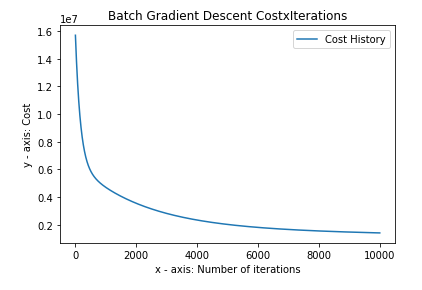
\includegraphics[scale=0.28]{images/smooth-gd-curve.png}
      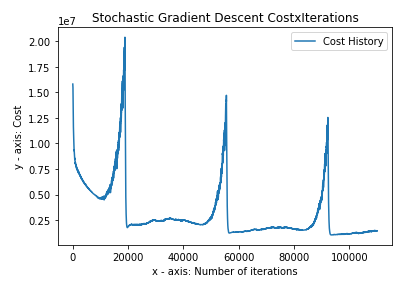
\includegraphics[scale=0.28]{images/steep-curves-in-stochastic-gd.png}
      \caption{Smooth curve and Stochastic unexpect curve due to outliers, respectively}
      \label{fig1}
  \end{figure}
	
    The outlier removal technique was based on the mean and standard deviation. Each sample's features should have its values falling in between the product of the feature's mean and its standard deviation. The described method was good enough to remove clear outliers (diamonds with a volume value equal to zero, for instance). Although, the stochastic curve presented the same behavior.
    
    After close analysis, the behavior was due to the data being ordered in an ascending order which was causing the unexpected behavior. After a simple shuffling of the data frame, the stochastically generated graphic was quite similar to the batch curve, as shown in Figure 2.
	
  \begin{figure}[!h]
      \centering
      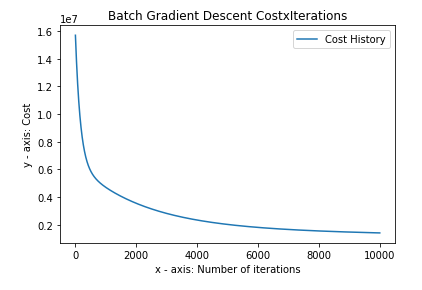
\includegraphics[scale=0.28]{images/smooth-gd-curve.png}
      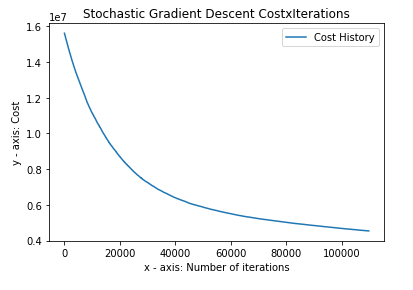
\includegraphics[scale=0.28]{images/smoother-curves-in-stochastic-gd.png}
      \caption{Smooth curve and Stochastic unexpect curve due to outliers, respectively}
      \label{fig1}
  \end{figure}
	
\section{Time and Accuracy Performance Tests}

	

\end{document}